\chapter{Related Work and Theory}
Inverse kinematics is applied in various fields, mainly robotics and computer
graphics. However, it is applied to a few unique problems, such as the
prediction of protein structure \cite{ccd_protein}. It has also found its uses in
rehabilitation medicine due to its miomechanical modelling ability. Over time,
many approaches have surfaced in order to solve the IK problem. There are
multiple families of solutions \cite{Aristidou2011} which suit different use
cases. Among others, trigonometric solutions can be used to solve certain IK
problems analytically, however, these solutions are often limited to solving two
bone IK scenarios. This paper will go over the iterative and heuristic
approaches which provide less complex solutions with the expansion of kinematic
chain lengths and degrees of freedom.

\section{Kinematics}
Kinematics is a branch of physics and a subdivision of classical mechanics
concerned with the geometrically possible motion of a body or system of bodies
without consideration of the forces involved \cite{kinematics_britannica}.
A kinematic chain is a tree like hierarchical structure of joint transforms
which are connected. Because the relationship between joints is hierarchical,
a transformation which is applied to a given joint affects all of its descendant
nodes. When manipulating a kinematic chain, transformations in the form of
rotations and translations are applied to joint transforms in order to achieve
a desired position of one or multiple transforms called the end effectors. The
problem of kinematics can be subdivided into two approaches which each present
their own problem and solution.

\begin{itemize}
    \item The problem of \textit{Forward Kinematics} which has to do with the
        identification of the final position of an end effector as a result of
        a set of transformations being applied to the kinematic chain to which
        the end effector belongs.
    \item The problem of \textit{Inverse Kinematics} which pertains to the
        search for a configuration of joint transformations for kinematic
        chain which allow the end effector to reach a predefined target
        position.
\end{itemize}

The forward kinematics (FK) problem can be said to have a guaranteed solution as
long as the set of joint transformations used as an input are known. To solve
the FK problem, the transformations are applied to the kinematic chain, and the
transform of the end effector is taken as an output. On the contrary, when
dealing with IK, the given problem may have no solutions, one solution, or many
solutions. 

\subsubsection{No Solutions}
An IK problem with no solutions can occur for several reasons. Most notably, and
IK solution is impossible when the target is unreachable through the limitations
of chain length. When the distance between the chain root and the target is
larger than the sum of distances between each adjacent chain link (Figure
\ref{fig:unreachable_dist1}), it is impossible to achieve a solution, as the
root of the chain is static and cannot be moved in order to allow the end
effector to reach its target. Similarly, and unreachable case exists if the
first bone segment is longer than the sum of the remaining bone segments (Figure
ref).

\begin{figure}[!h]
    \centering
    \captionsetup{justification=centering}
    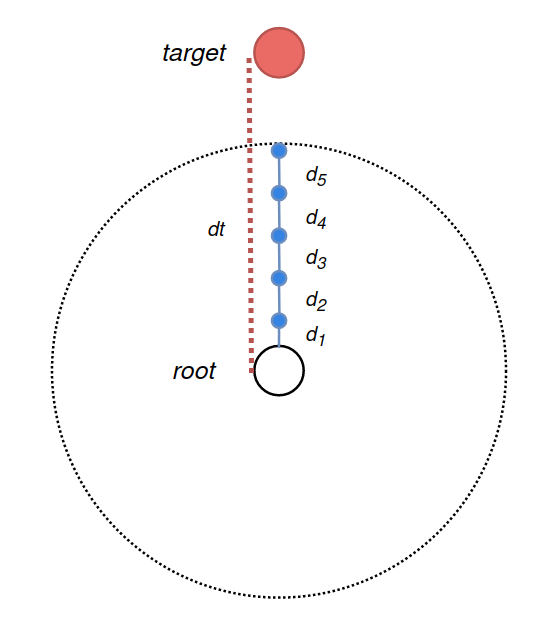
\includegraphics[width=0.5\textwidth]{grafika/unreachable_dist_1.png}
    \caption{An IK problem with no solution where the target is unreachable
    because the sum of segment distances is less than the distance between the
    root and the target \(\sum_{i=1}^{n}d_i < dt\) }
    \label{fig:unreachable_dist1}
\end{figure}

\begin{figure}
    \centering
    \captionsetup{justification=centering}
    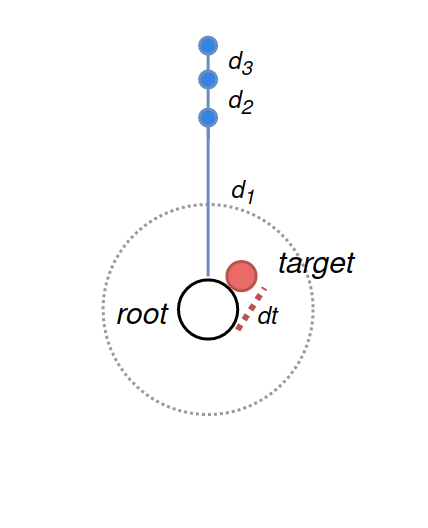
\includegraphics[width=0.4\textwidth]{grafika/unreachable_dist_2.png}
    \caption{An IK problem with no solution where the target is unreachable
    because the length of the first segment is greater than the summed length of
    the rest of the kinematic chain \(d_1 - \sum_{i=2}^{n}d_i > dt\). This creates
    a radius around the root where if its distance to the target is smaller, it
    indicates an unreachable target.  } \label{fig:unreachable_dist2}
\end{figure}

Another reason for the lack of solutions to an IK problem can be the
over-constraining of the problem. Constraints in an IK problem are used to
dictate the range of motion that each joint. Constraints might limit the joint's degrees of
freedom by reducing the dimensions in which it can perform its rotational and
translational transformations. Such constraints are often modelled after joints
which are present in the domain of biomechanics, such as hinge joints, ball
joints, pivot joints. A constraint can also limit the extent of a joint's
ability to bend which is defined by the allowed angle of the joint's rotation in
relation to the rotation of its parent node. If too many of such constraints are
added to a kinematic chain, it may have blind spots for which it is unable to
find a configuration of transformations which can bend the chain to reach the
target.

\begin{figure}
    \centering
    \captionsetup{justification=centering}
    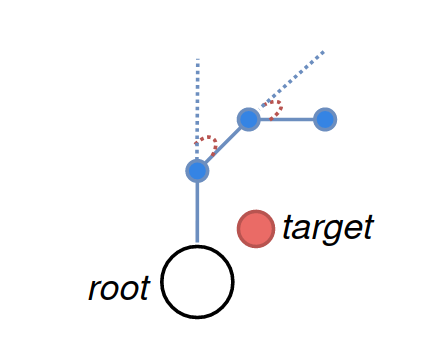
\includegraphics[width=0.4\textwidth]{grafika/unreachable_angles.png}
    \caption{An IK problem with no solution where the rotational constraints
    placed on the joints prevent the end effector from being able to bend enough
    to reach the target}
    \label{fig:params}
\end{figure}

\subsubsection{One or many solutions}
When an IK problem is not limited by the cases mentioned above, it can have one,
or many solutions depending on the case and constraints. More often than not the
problem will have multiple available solutions, and if the kinematic chain is
unconstrained, the solution set for and IK problem grows very large.

While the introduction of constraints can increase the cases for which an IK
problem has only one solution, the simplest case to consider for an
unconstrained kinematic chain is one where the chain must stretch to its full
extent in order to reach the target. The sum of the chain's segment lengths
\(d_i\) is equal to the distance from the root to the target \(dt\).
\[
    \sum_{i=1}^{n}d_i = dt
    \]

\section{IK Algorithms}
